\chapter{Преглед на предметната област} % Main chapter title

\label{Chapter2} 

%----------------------------------------------------------------------------------------

\section{Въведение}
Изграждането на отворена диалогова система е предизвикателна задача, с която са се сблъсквали много екипи. През годините са опитвани различни подходи за изграждане на подобна система и в тази глава ще се запознаем с основните методи и тяхната еволюция. 
Благодарение на прогреса в сферата на машинното самообучение и на нарастващата изчислителна мощ бяха постигнати подобрения в задачата за автоматичен машинен превод. Ще обобщим тяхната архитектура и ще коментираме приложимостта на подобен модел за изграждане на диалогова система.
Ще разгледаме и проблема за отговаряне на често задавани въпроси и връзката му с диалоговите системи


https://research.fb.com/the-long-game-towards-understanding-dialog/

\section{Диалогови системи: мотивация и история}

Диалоговите системи са ултимативния интерфейс за употреба на компютърно устройство. Комуникацията с машина не трябва да бъде по-различна от комуникацията с друг човек. Постигането на тази цел ще направи устройствата по-достъпни и потребителите по-склонни да ги направят част от ежедневния си живот. \\
Идеята за диалогова система датира още от зората на компютърната индустрия. В следващите секции ще представим различните стадии на развитие на диалогови системи през годините.

\subsection{ELIZA}
ELIZA \cite{eliza} е първата известна диалогова система. Разговорите с ELIZA симулират интервю с психотерапевт. Тъй като при такова интервю целта е потребителят да разкаже за собствения си мироглед, програмата няма нужда от знания за обиколния свят. Достатъчно е да бъде пасивна и да рефлектира на репликите на потребителя, насърчавайки го да разкаже повече за себе си. \\ Системата разчита на правила, които определят нейното поведение. Всяко правило се състои от ключова дума, тежест на ключовата дума и рецепта за трансформиране на входните данни в изходни. Едно примерно правило изглежда така:

\begin{verbatim}
["remember", 5, [
["* i remember *", [
"Do you often think of (2) ?",
"Does thinking of (2) bring anything else to mind ?",
"What else do you recollect ?",
"Why do you remember (2) just now ?",
"What in the present situation reminds you of (2) ?",
"What is the connection between me and (2) ?",
"What else does (2) remind you of ?"
]],
\end{verbatim}

При новопостъпило съобщение ELIZA извлича думата с най-голяма тежест и преобразува входните данни спрямо правилото на съответната дума. Примерен разговор с ELIZA може да се намери във фигура \ref{eliza-image}.
\begin{figure}
	\caption{Примерен разговор с ELIZA}
	\label{eliza-image}
	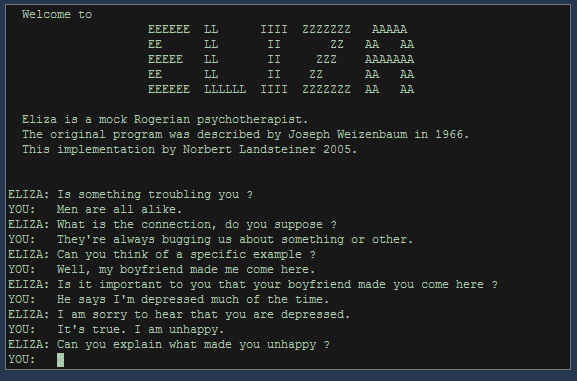
\includegraphics{eliza.png}[caption="ELIZA"] 
\end{figure}

Макар и да е базирана на прости правила, ELIZA е била доста иновативна за времето си. Някои потребители са я определяли като интелигентна и са й приписвали човешки чувства. 
\subsection{PARRY}
PARRY \cite{parry} e първата диалогова система, която минава теста на Туринг\cite{turing}. PARRY е създаден да симулира човек страдащ от параноя.  \\
Иновативното в архитектурата на PARRY e че той има променливо състояние, което кодира мнението му за себе си и за партньора му. В зависимост от това състояние, PARRY дава различни отговори. Друга разлика е че PARRY има лична история, която e склонен да разкаже, стига нивото му на параноя да не е твърде високо.
\subsection{ALICE}
\subsection{games}

\subsection{assistants}
\subsection{commercial}
But the chatbots on Facebook Messenger and other apps such as Kik, Telegram, Slack and WeChat aren’t dreaming of electric sheep. Rather than trying to pass for human, they’re unashamedly artificial, and focused entirely on providing information and/or completing tasks for the humans they interact with. If they have views on Brexit, they’re not letting on.

\section{Машинен превод}
- statistical machine translation
- neural machine translation
- seq2seq
- seq2seq with attention

\section{Отговаряне на често задавани въпроси}
- проблем
- решение

